\documentclass[12pt,twoside]{report}
\usepackage[utf8]{inputenc} % set encoding to UTF8
\usepackage[T1]{fontenc} % more info visit : https://tex.stackexchange.com/questions/664/why-should-i-use-usepackaget1fontenc
\usepackage{graphicx} % package to load images
\usepackage[french]{babel} % set language to french
\usepackage{titlesec} % customise the look of the start of the chapters
\usepackage[a4paper,width=150mm,top=25mm,bottom=25mm,bindingoffset=6mm]{geometry} % set papersize and margins
\setlength{\headheight}{14.49998pt} % needed for fancyhdr
\usepackage{fancyhdr} % add headers and footers 
\pagestyle{fancy} % header type
\renewcommand{\chaptermark}[1]{% set custom header 
\markboth{\MakeUppercase{ #1}}{}} % set default style of the header more details visit : https://mirror.marwan.ma/ctan/macros/latex/contrib/fancyhdr/fancyhdr.pdf Page 19
\fancyfoot{} % set footer
\renewcommand{\footrulewidth}{0.3pt}% % set line before footer
\fancyfoot[LE,RO]{\tiny{ENSIAS}} % LE left EVEN RO Right ODD write ENSIAS
\fancyfoot[lo,RE]{\thepage} % write the page number
\usepackage{caption} % for captioning
\usepackage{subcaption} % for multiple figs 
\usepackage{biblatex} % for references
\addbibresource{ref.bib} % set file with refs
\usepackage{csquotes} % biblatex recommend it
\usepackage{lipsum} % generate dummy text
% set metadata
%\usepackage{xmpincl}
%\includexmp{meta.xmp} 
% set default path to images
\graphicspath{ {Images/} } 


% set title
\title{application Web/Mobile de suivi de Budget }
% set custom look to every chapter
% more details visit : https://www.overleaf.com/learn/latex/Sections_and_chapters
\titleformat
{\chapter} % command
[display] % shape
{\bfseries\Large} % format
{} % label
{0.1ex} % sep
{
  %  \rule{\textwidth}{1pt}
   % \vspace{1ex}
} % before-code
[
\vspace{-0.5ex}%
\rule{\textwidth}{0.3pt}
] % after-code

% rename tables
%\renewcommand*\contentsname{Table des matieres}
%\renewcommand{\listfigurename}{List des Figures}
%\renewcommand{\listtablename}{Liste des tables}

\begin{document}
% title page    
\begin{titlepage}
    \begin{minipage}[t]{0.2\textwidth}    %% b or t, default is c
        
\includegraphics[width=\linewidth]{ensias.png}
    \end{minipage}%
  \begin{minipage}[t][2cm]{0.6\textwidth}
    \centering\bfseries\large
    \hfill
  \end{minipage}%
    \begin{minipage}[t]{0.2\textwidth}
    
\includegraphics[width=\linewidth]{um5.png}
  \end{minipage}
  \begin{center}
  \vspace{0.2cm}
  {\huge Ecole Nationale Supérieure d’Informatique et d’Analyse des Systèmes}\\
  \vspace{0.5cm}
  \textbf{FILIERE : GENIE LOGICIEL}
  \vspace{0.5cm}
  \hrule
  \vspace{0.2cm}
  \textbf{\huge application Web/Mobile de suivi de Budget}
  \vspace{0.5cm}
  \hrule
  \vspace{1.5cm}
  \vfill
  \begin{minipage}[t]{0.45\textwidth}    %% b or t, default is c
        \textit{Realise par :}\\

        BAKHOUCH Nisrine\\
        EL BOUZIYANI Anas
    \end{minipage}%
    \begin{minipage}[t]{0.45\textwidth}    %% b or t, default is c
        \textit{Sous la direction de :}\\
        
        Pr EL HAMLAOUI Mahmoud
    \end{minipage}%
       \vspace{1.8cm}
       Department Informatique\\
       ENSIAS - UM5\\
       Année Académique 2023/2024
   \end{center}
\end{titlepage}
% add a blank page
\shipout\null
\stepcounter{page} % in order to count for the blank page
%-- les differents parties --
\chapter{Remerciments} % add or remove * to enable/disable numbering
Au terme de ce projet nous exprimons notre profonde gratitude envers notre encadreur Pr.EL HAMLAOUI Mahmoud pour sa vigilance constante  et ses remarques constructives qui ont enrichi notre travail. Nous le remercions chaleureusement pour sa disponibilité et son précieux accompagnement, et nous avons été honorés de bénéficier de ses directives et  ses conseils éclairés tout au long du projet. 



\chapter{Resume} % add or remove * to enable/disable numbering
Notre projet académique de fin d'année se concentre sur le développement d'une application mobile dédiée à la gestion de syndic de copropriété afin d'optimiser les processus existants et de renforcer la transparence des opérations.
Pour atteindre ces objectifs, une approche Agile, en particulier la méthodologie Scrum , a été adoptée pour gérer le projet de manière itérative.
En termes de développement nous avons utilise les meilleures pratiques de developpement logiciel et les technologies modernes tells que  Android Jetpack Compose pour le développement de l'interface utilisateur, Gradle pour la gestion de build, Firebase pour les services backend et UML pour la conception.
Le resultat final est une application mobile fonctionnelle offrant une interface utilisateur intuitive et conviviale.


\chapter{Abstract} % add or remove * to enable/disable numbering
The main focus of our academic project is the development of a mobile application for managing a joint property in order to optmize the existing processes of budget managing and enforce the transparency of operations. In order to achieve our goals, we opted for a Scrum/Agile approach, Meanwhile we used the latest technologies (Android JetPack Compose for ui, MVVM as a model, Firebase for backend...) the end result is a fully functional application

\vfill
\hrule
\vspace{0.5cm}
\textbf{Keywords : } Agile, Application, Android, Dagger-Hilt, Firebase, Gradle, JetPack-Compose, Mobile, Scrum, UML.
\vspace{0.5cm}
\hrule


\tableofcontents % table des matieres
\listoffigures % table des figures
\listoftables % table des tableau

\chapter{Introduction} % add or remove * to enable/disable numbering
TO BE IMPLEMENTED



\chapter{Chapitre 1} % add or remove * to enable/disable numbering
\section{Problematique}
\lipsum[2-2]
\section{Solution}
\lipsum[2-2]
\section{Analyse des besoins}
\lipsum[2-2]
\subsection{Besions fonctionnels}
\lipsum[2-2]
\subsection{Besoins non fonctionnels}
\lipsum[2-2]
\section{Objectifs}
\lipsum[2-2]

\appendix

\addcontentsline{toc}{chapter}{ Bibliographie}
\printbibliography

\chapter{annexes} % add or remove * to enable/disable numbering

\begin{figure}[h]
    \centering
    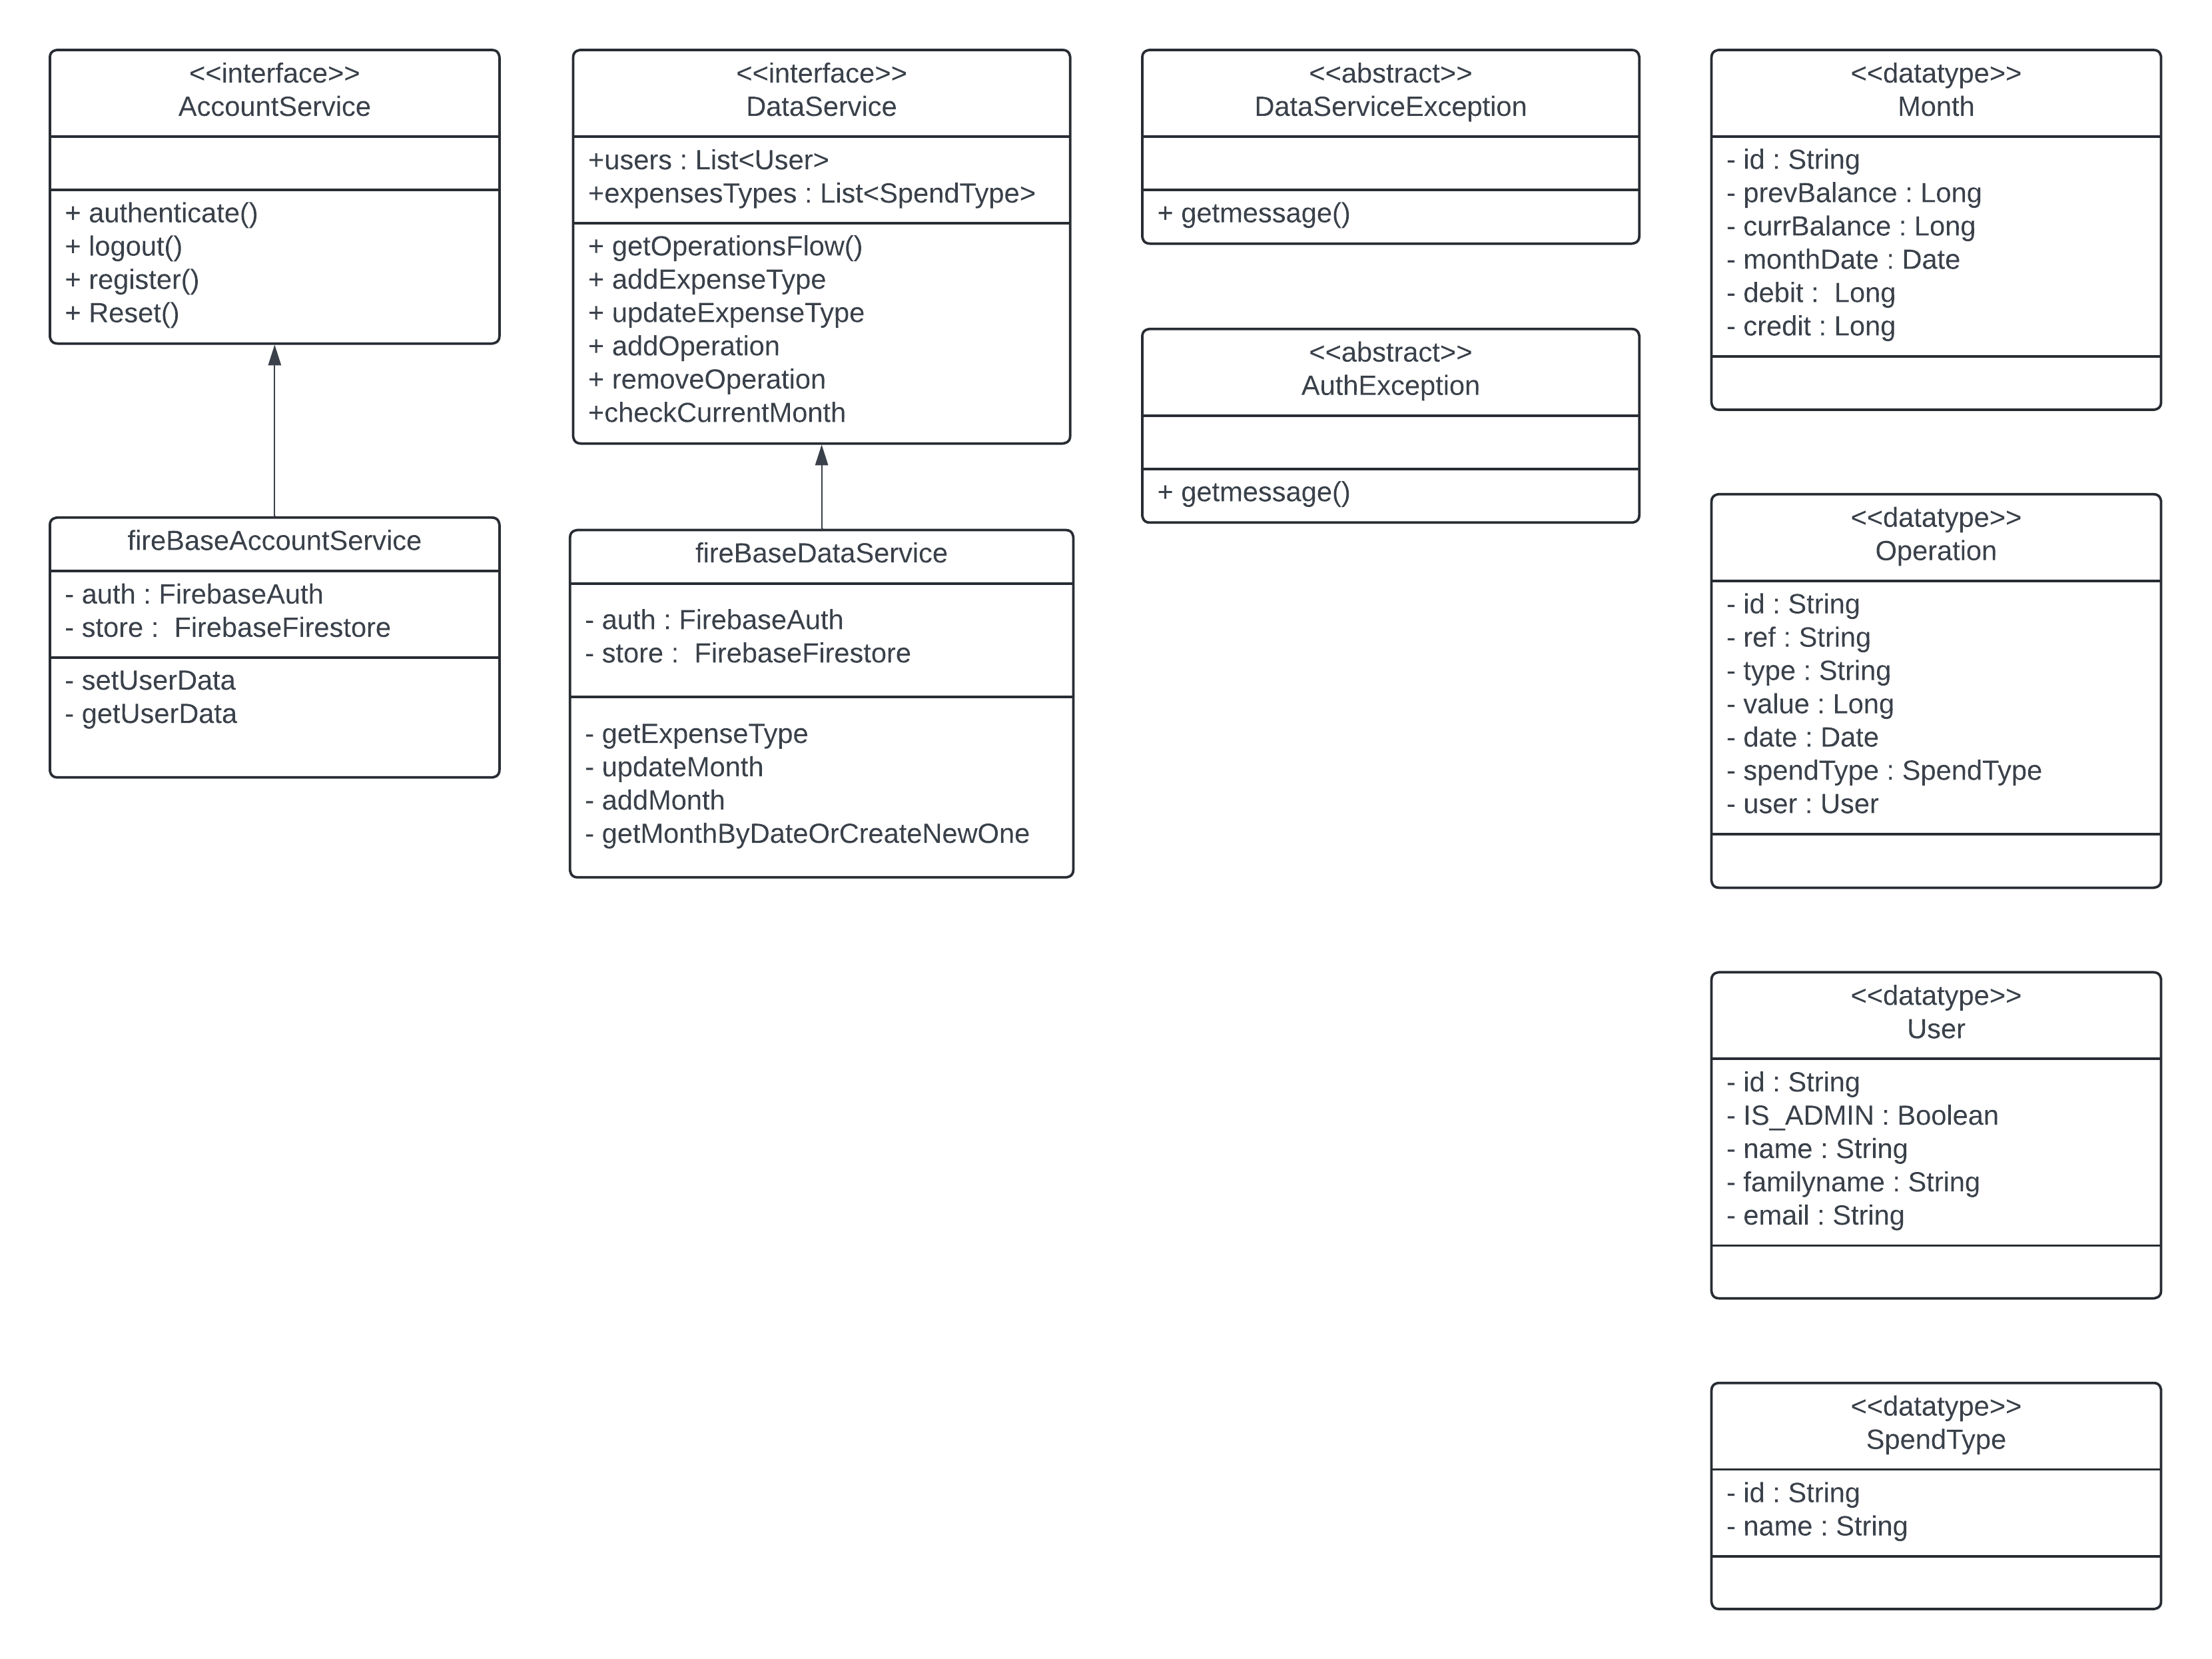
\includegraphics[width=1\textwidth]{diag classe metier.png}
    \caption{Diagramme de classe métier}
\end{figure}


list des products backlog

\begin{figure}[h]
    \centering
    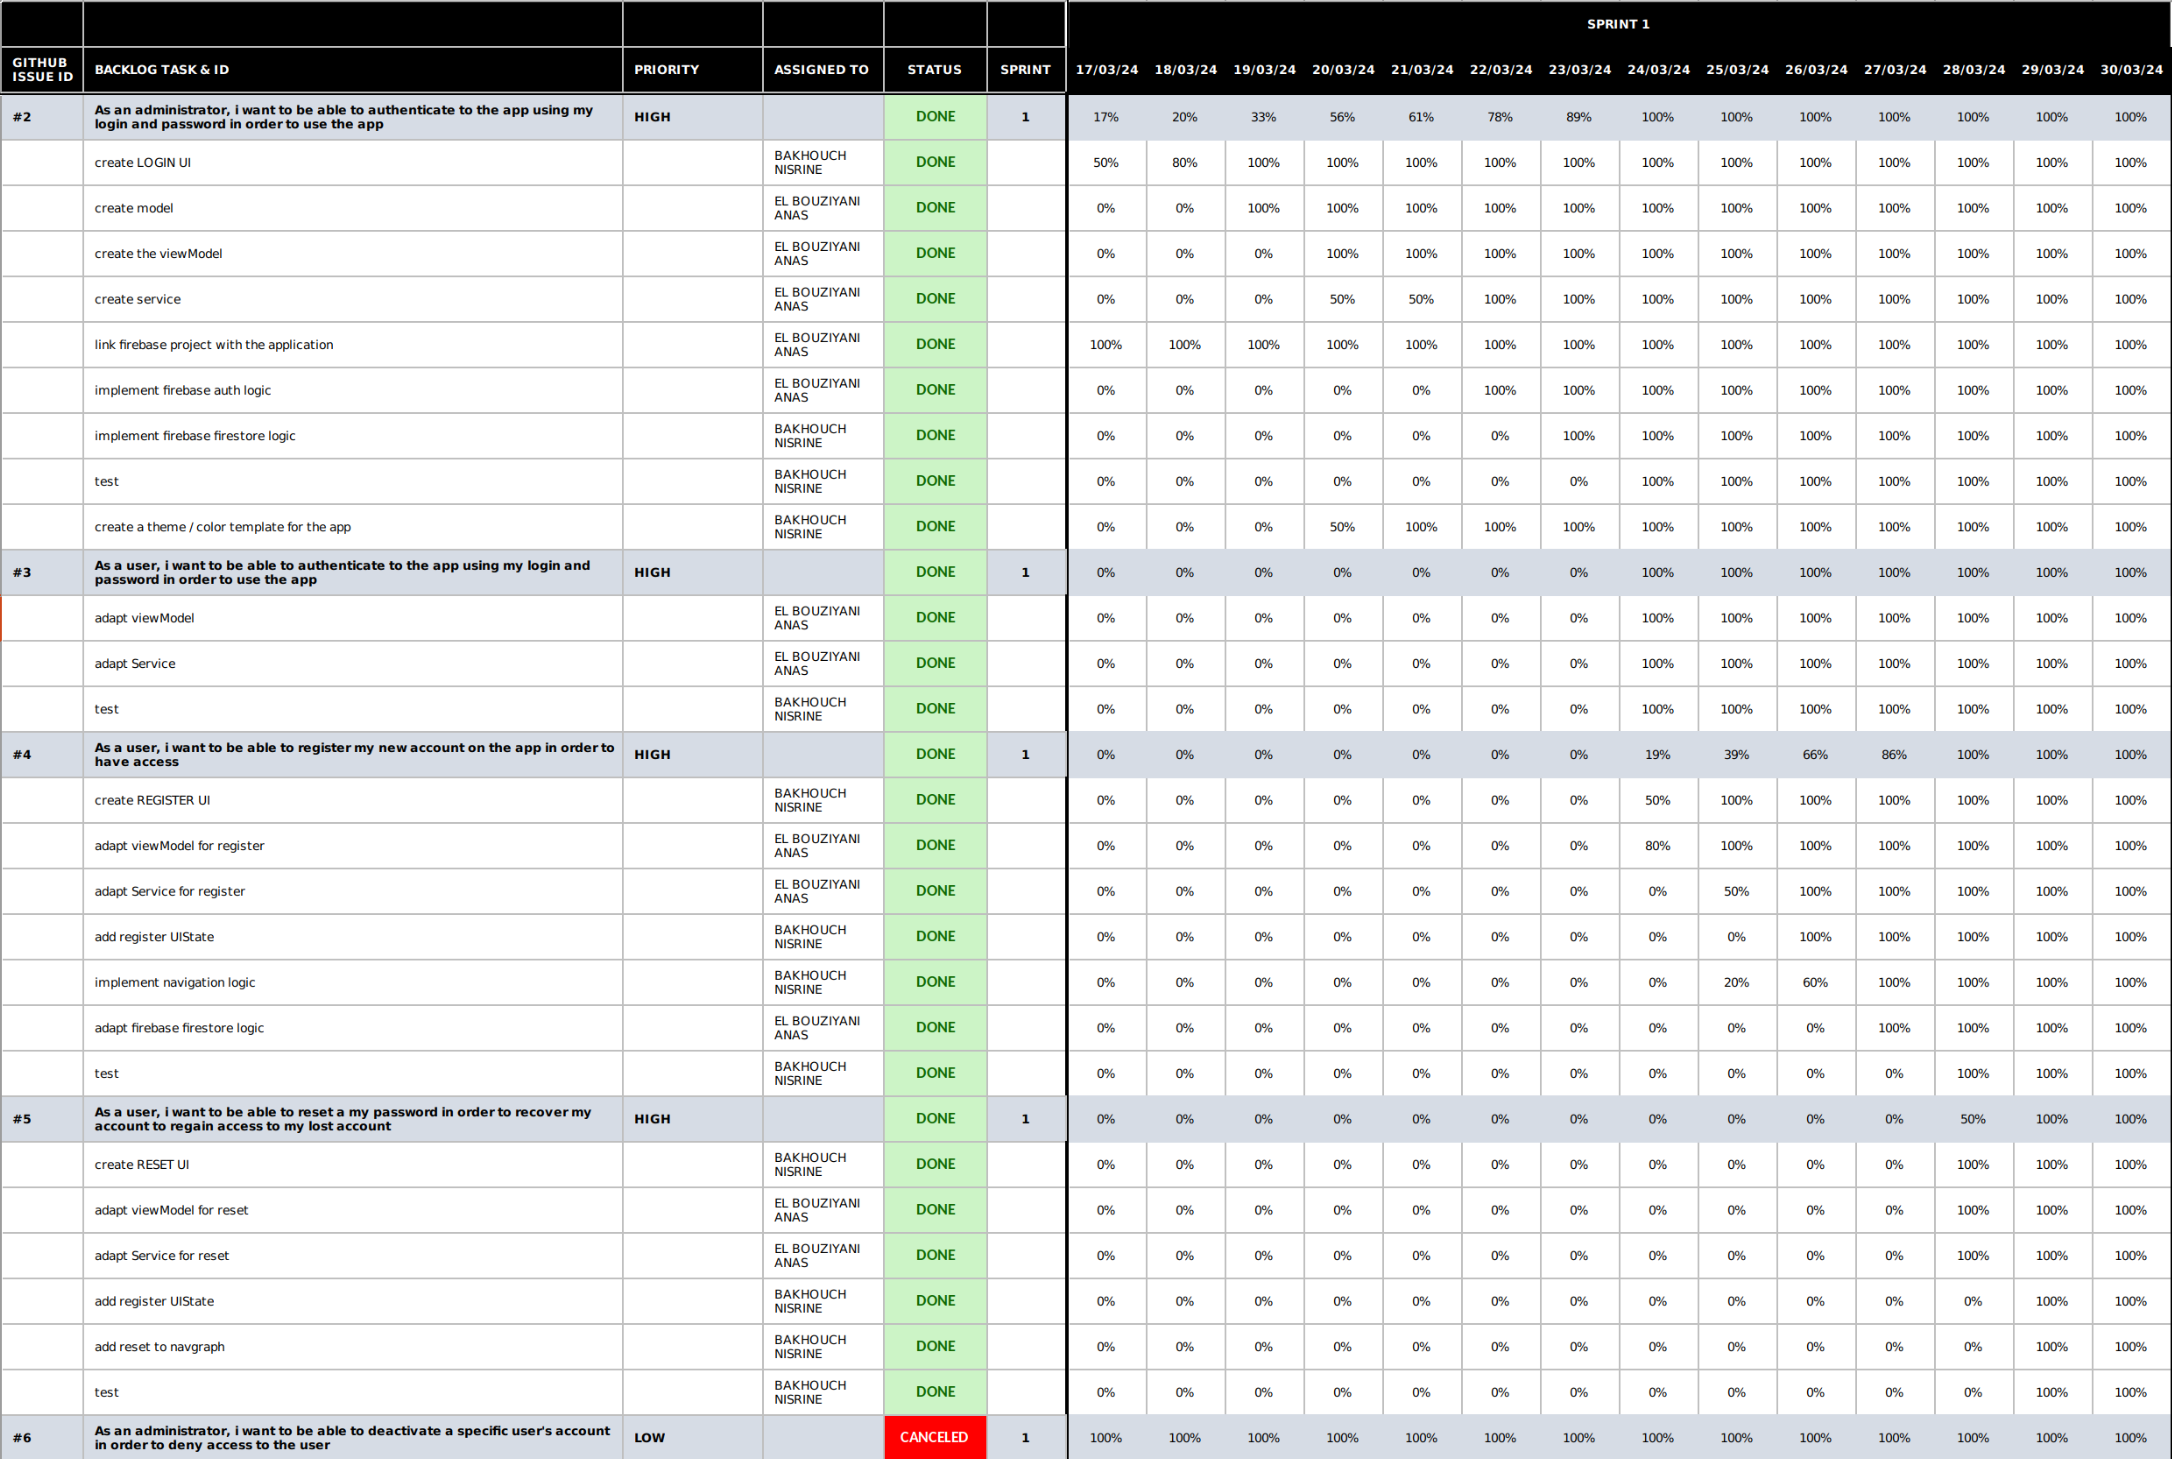
\includegraphics[width=1\textwidth]{sprint1.png}
    \label{Sprint1}
    \caption{Product Backlog de sprint 1}
\end{figure}


\begin{figure}[h]
    \centering
    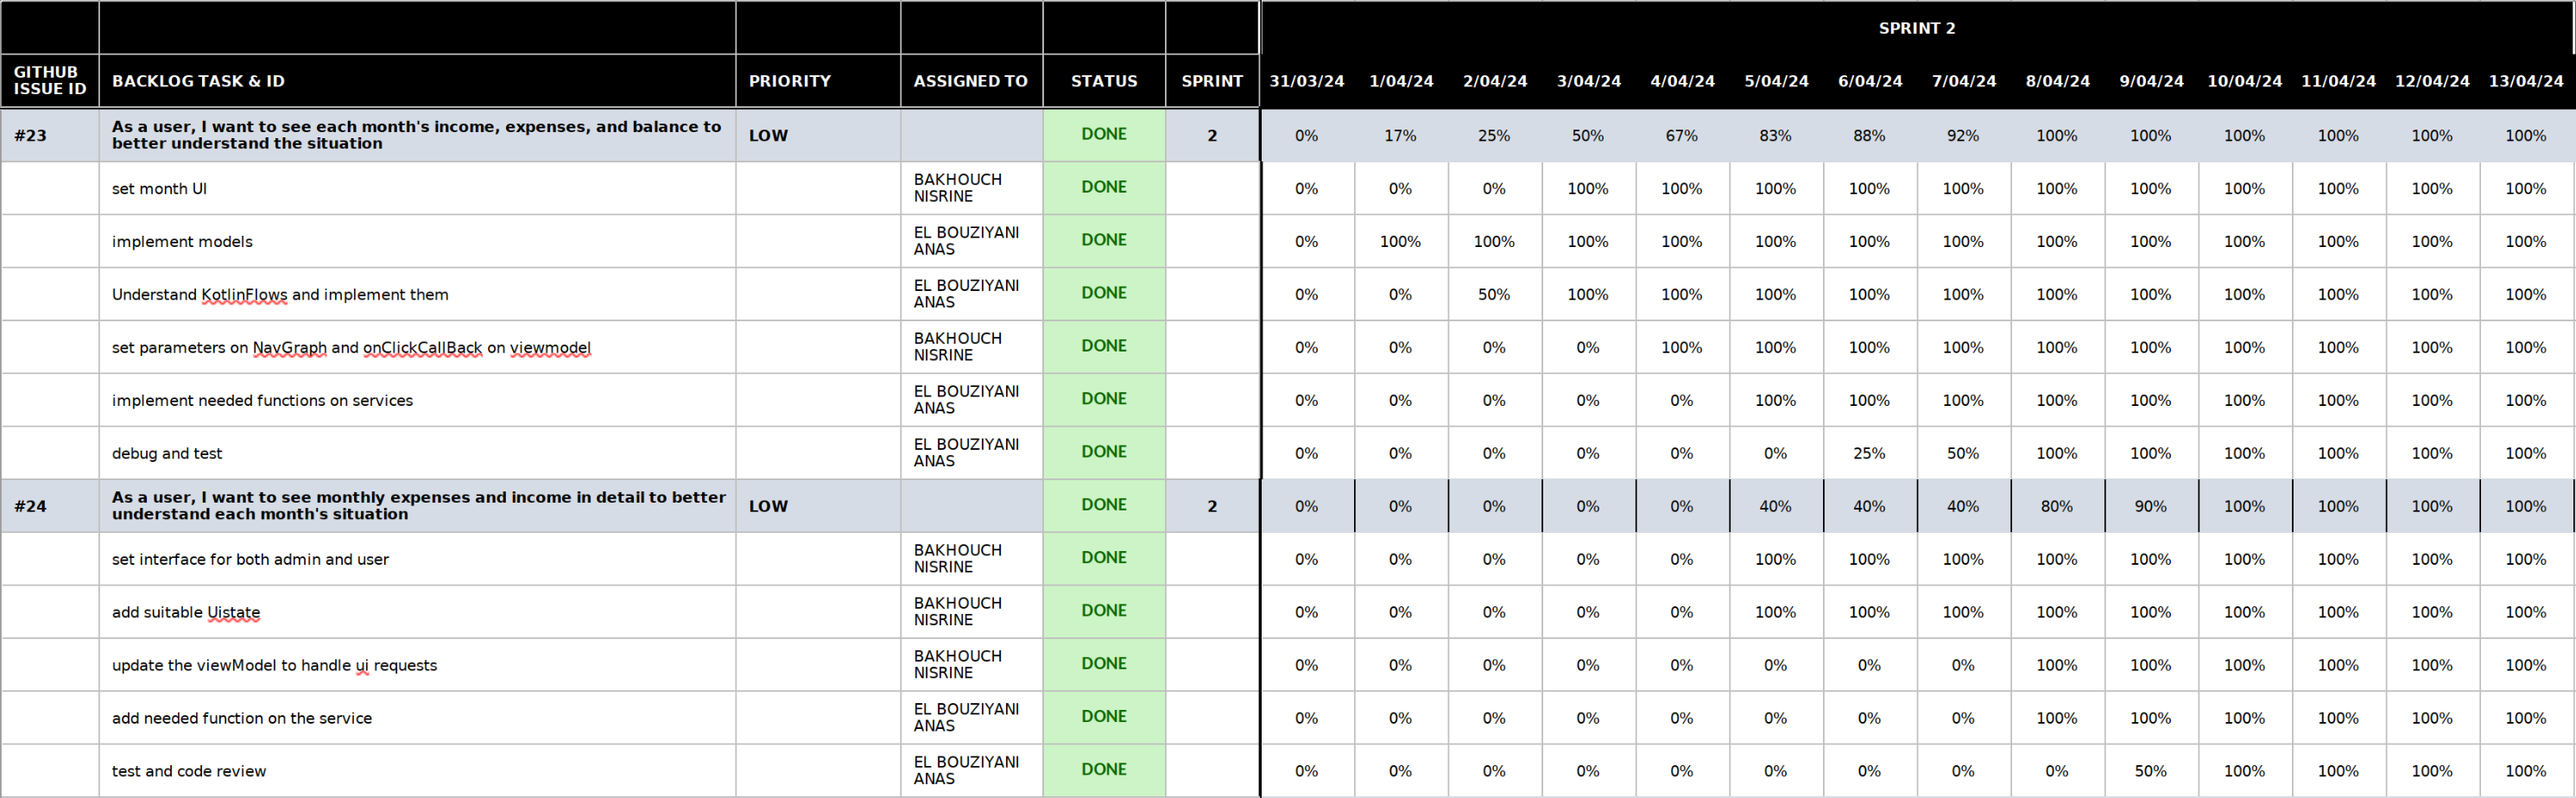
\includegraphics[width=1\textwidth]{sprint2.png}
    \label{Sprint2}
    \caption{Product Backlog de sprint 2}
\end{figure}


\begin{figure}[h]
    \centering
    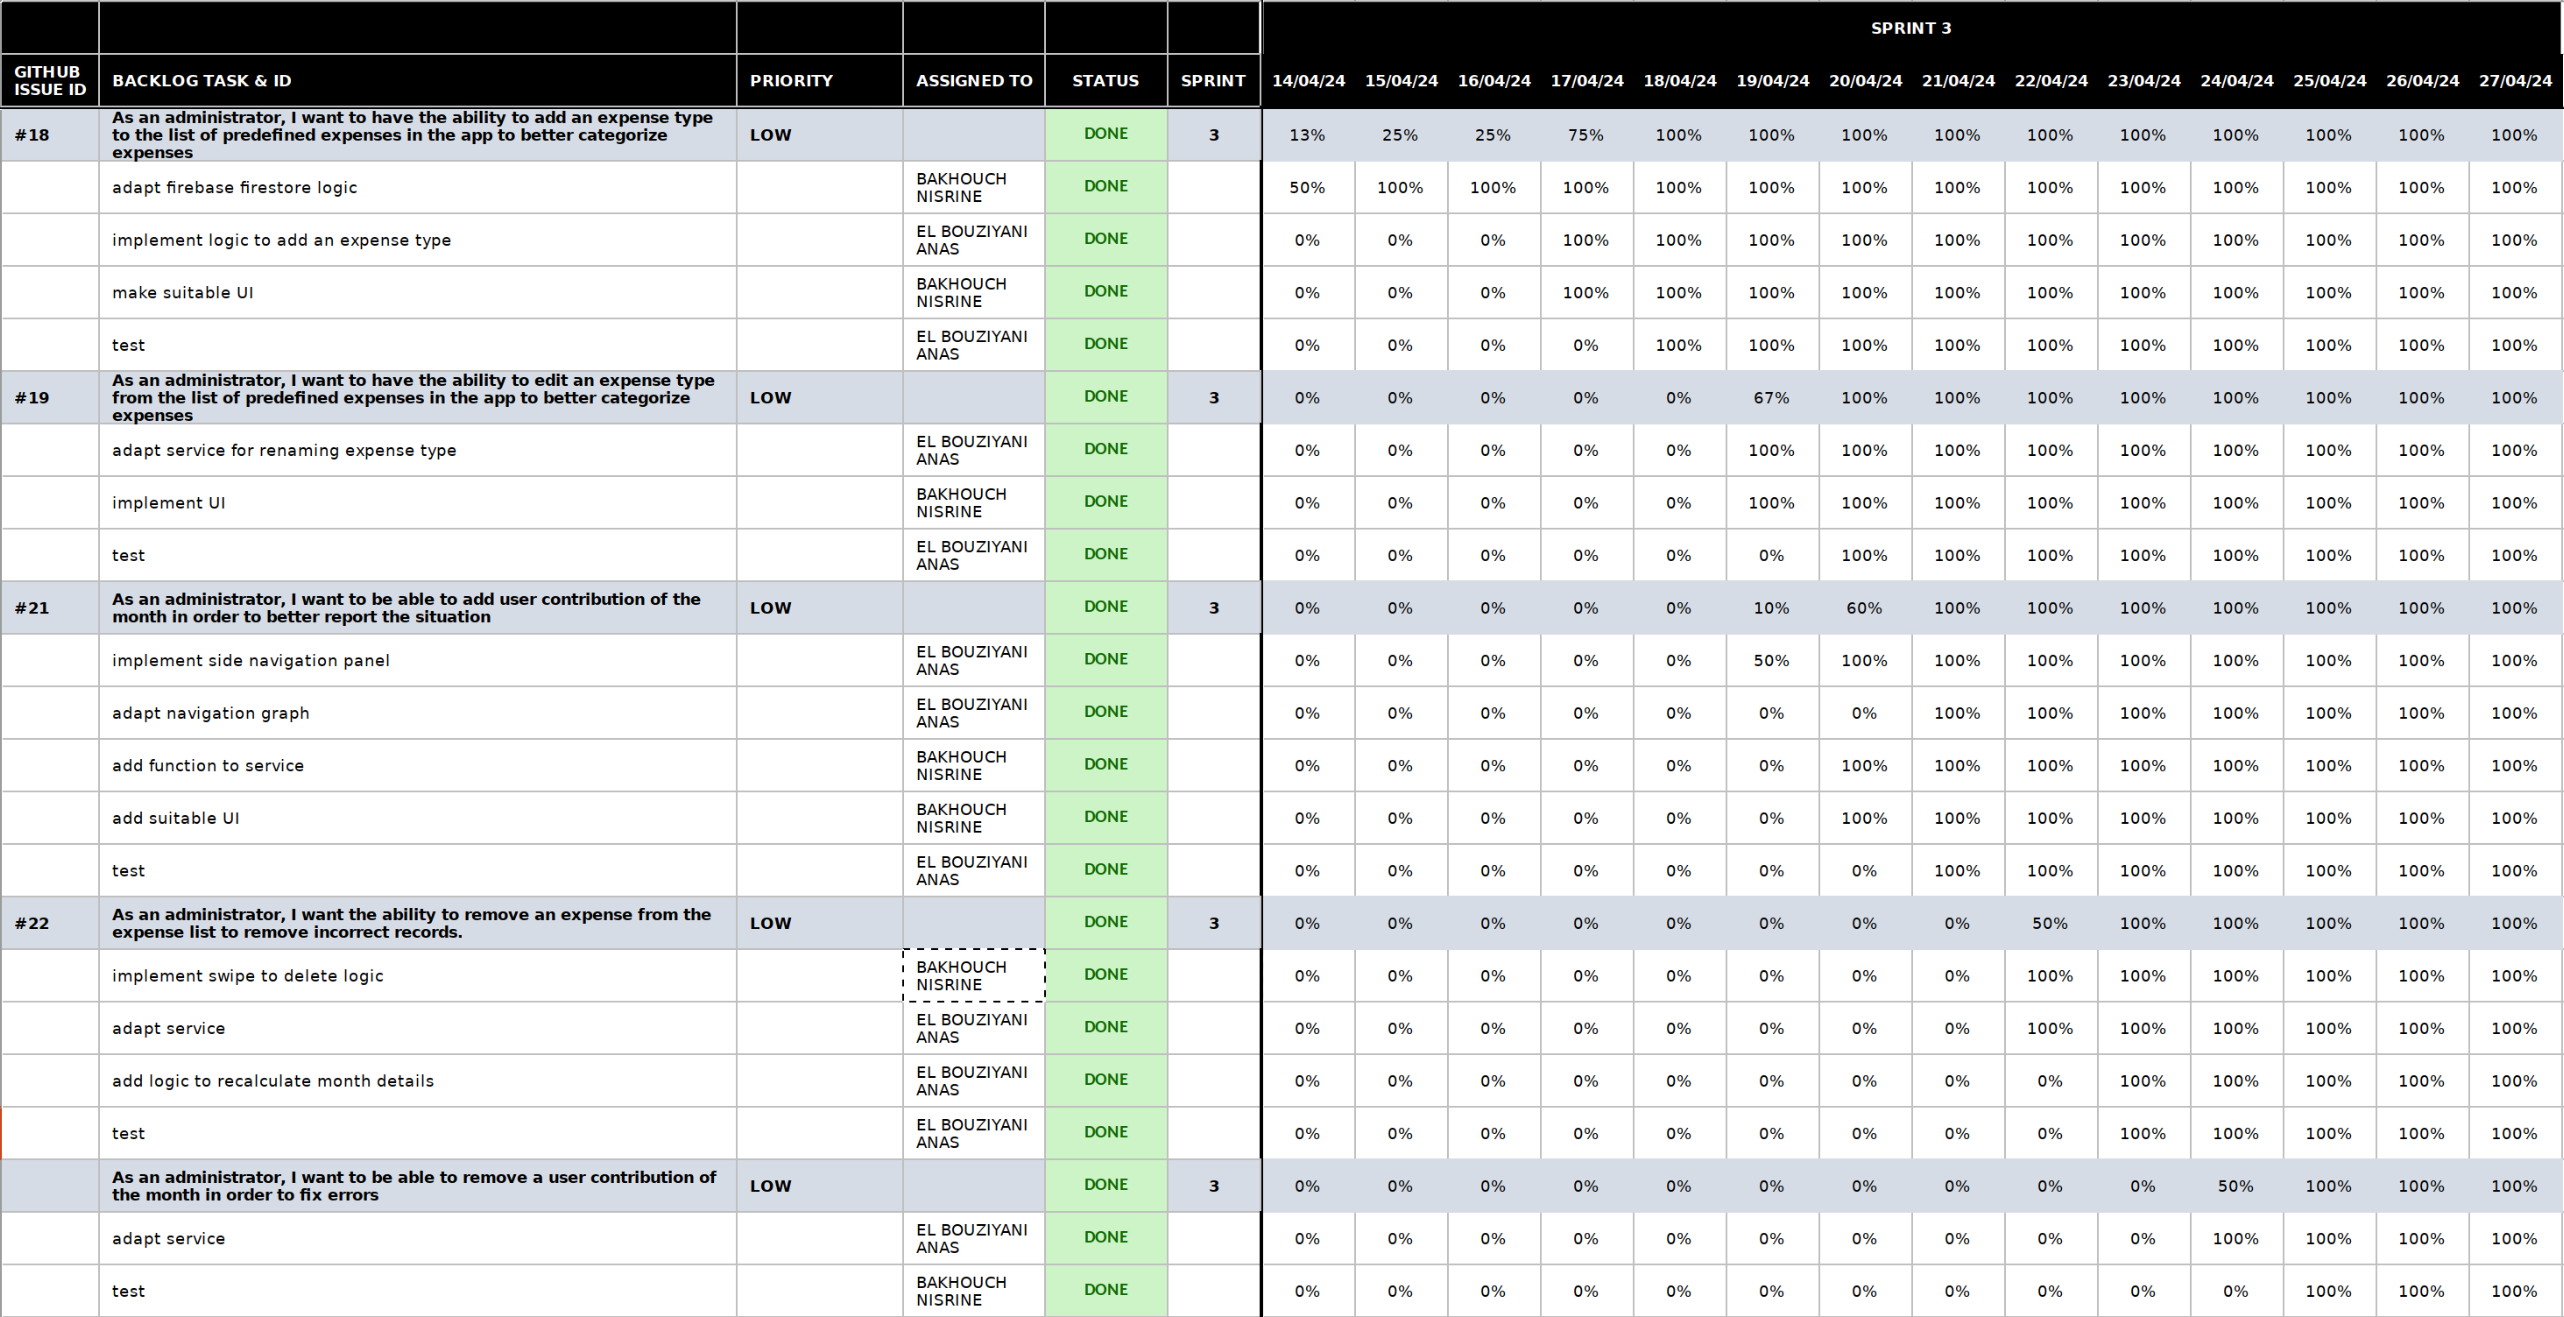
\includegraphics[width=1\textwidth]{sprint3.png}
    \label{Sprint3}
    \caption{Product Backlog de sprint 3}
\end{figure}






\end{document}
